\documentclass{standalone}
    \usepackage{tikz}
    \usepackage{amssymb}
    \usetikzlibrary{shapes.geometric, shapes.misc}
    \usetikzlibrary{automata, positioning}

    \begin{document}
    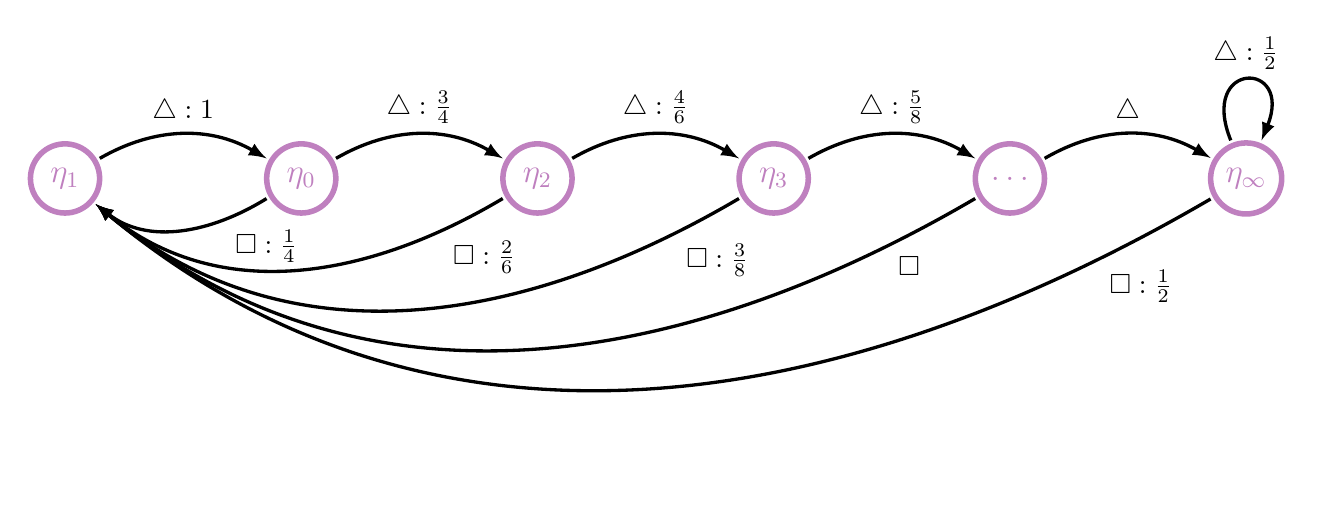
\begin{tikzpicture}[node distance=3cm,
        % bend angle=15, 
        auto,
        every loop/.style={},
        %,line width=1.2
        every edge/.style={->,draw=black,>=latex,shorten <=1pt, shorten >=1pt},
        every state/.style={draw=black,line width=2,font=\large},
        loop right/.style={right,out=22,in=-22,loop},
        loop above/.style={above,out=112,in=68,loop},
        loop left/.style={left,out=202,in=158,loop},
        loop below/.style={below,out=292,in=248,loop},
        loop above right/.style={right,out=67,in=23,loop},
        loop above left/.style={left,out=157,in=113,loop},
        loop below left/.style={left,out=247,in=203,loop},
        loop below right/.style={right,out=337,in=293,loop},
        binode/.style={minimum size=1cm,inner sep=0pt},]


        \node[state, red!50!blue!50] (n_1) {$\eta_1$};
        \node[state, red!50!blue!50] (n_0) [right of = n_1] {$\eta_0$};
        \node[state, red!50!blue!50] (n_2) [right of=n_0] {$\eta_2$};
        \node[state, red!50!blue!50] (n_3) [right of=n_2] {$\eta_3$};
        \node[state, red!50!blue!50] (n_dots) [right of=n_3] {$\dots$};
        \node[state, red!50!blue!50] (n_inf) [right of=n_dots] {$\eta_{\infty}$};

        \path[->, line width=1.2] (n_1) edge [bend left] node {$\triangle : 1 $} (n_0);       

        \path[->, line width=1.2] (n_0) edge [bend left, in=140] node[pos=0.25] {$\square : \frac{1}{4}$} (n_1);
        \path[->, line width=1.2] (n_0) edge [bend left] node {$\triangle : \frac{3}{4}$} (n_2);

        \path[->, line width=1.2] (n_2) edge [bend left, in=140] node[pos=0.15] {$\square : \frac{2}{6}$} (n_1);
        \path[->, line width=1.2] (n_2) edge [bend left] node {$\triangle : \frac{4}{6}$} (n_3);

        \path[->, line width=1.2] (n_3) edge [bend left, in=140] node[pos=0.1] {$\square : \frac{3}{8}$} (n_1);
        \path[->, line width=1.2] (n_3) edge [bend left] node {$\triangle : \frac{5}{8}$} (n_dots);

        \path[->, line width=1.2] (n_dots) edge [bend left, in=140] node[pos=0.1] {$\square$} (n_1);
        \path[->, line width=1.2] (n_dots) edge [bend left] node {$\triangle$} (n_inf);

        \path[->, line width=1.2] (n_inf) edge [bend left, in=140] node[pos=0.1] {$\square : \frac{1}{2}$} (n_1);
        \path[->, line width=1.2] (n_inf) edge [loop above] node {$\triangle : \frac{1}{2}$} (n_inf);
        
    \end{tikzpicture}
    \end{document}